%%
%% Class homework & solution template for latex
%% Alex Ihler
%%
\documentclass[twoside,11pt]{article}
\usepackage{amsmath,amsfonts,amssymb,amsthm}
\usepackage{graphicx,color}
\usepackage{verbatim,url}
\usepackage{listings}
\usepackage{hyperref}
\usepackage{upquote}
\usepackage[T1]{fontenc}
%\usepackage{lmodern}
\usepackage[scaled]{beramono}
%\usepackage{textcomp}

% Directories for other source files and images
\newcommand{\bibtexdir}{../bib}
\newcommand{\figdir}{fig}

\newcommand{\E}{\mathrm{E}}
\newcommand{\Var}{\mathrm{Var}}
\newcommand{\N}{\mathcal{N}}
\newcommand{\matlab}{{\sc Matlab}\ }

\setlength{\textheight}{9in} \setlength{\textwidth}{6.5in}
\setlength{\oddsidemargin}{-.25in}  % Centers text.
\setlength{\evensidemargin}{-.25in} %
\setlength{\topmargin}{0in} %
\setlength{\headheight}{0in} %
\setlength{\headsep}{0in} %

\renewcommand{\labelenumi}{(\alph{enumi})}
\renewcommand{\labelenumii}{(\arabic{enumii})}

\theoremstyle{definition}
\newtheorem{MatEx}{M{\scriptsize{ATLAB}} Usage Example}

\definecolor{comments}{rgb}{0,.5,0}
\definecolor{backgnd}{rgb}{.95,.95,.95}
\definecolor{string}{rgb}{.2,.2,.2}
\lstset{language=Matlab}
\lstset{basicstyle=\small\ttfamily,
        mathescape=true,
        emptylines=1, showlines=true,
        backgroundcolor=\color{backgnd},
        commentstyle=\color{comments}\ttfamily, %\rmfamily,
        stringstyle=\color{string}\ttfamily,
        keywordstyle=\ttfamily, %\normalfont,
        showstringspaces=false}
\newcommand{\matp}{\mathbf{\gg}}




\begin{document}

\subsection{Mixed Dimensional Mesh}

Here I show the cooling and heating effects of a rod on a plate. Here is the initial mesh:
**REPLACE MESH**
\begin{figure}[h]
\centering
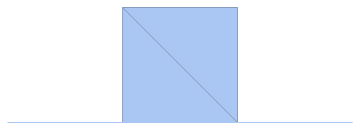
\includegraphics[width=3 in]{mixedMeshPic.png}
\caption{A line and square joined together}
\end{figure}
\\
The topological space has 3 strata: \\
1) The left rod\\
2) The right rod\\
3) The square

\subsection{Studying the square}

The square will have a heat equation $v(x,y,t)$. \\
Here is the square's diffusion equation:
\[
\alpha_1 (\frac{\partial^2 v}{\partial x^2} + \frac{\partial^2 v}{\partial y^2}) = \frac{\partial v}{\partial t}
\]
This is the initial condition:
\[
v(x,y,0) = -20x(x-1.5)(x-3)y(y-1)
\]
The boundary conditions are as follows:
\[
v(0,y,t)=0
\]
\[
v(3,y,t)=0
\]
\[
v(x,0,t)=0
\]
\[
v(x,1,t)=0
\]

\subsection{Square without the rod}

For this case, I solved the above differential equation system **WRITE MORE IF POSSIBLE**
\newpage
\subsection{Heat Equation Over Rod}

The heat equation for the rods $u(y,t)$ is as follows:
\[
\alpha_1 \frac{\partial^2 u}{\partial y^2} = \frac{\partial u}{\partial t}
\]
The boundary conditions will be as follows:
\[
u(0,t)=0
\]
\[
u(3,t)=0
\]
The initial condition for the left rod is as follows:
\[
u_1(y,0)=y(y-1)
\]
The initial condition for the right rod is as follows:
\[
u_2(y,0)=-y(y-1)
\]

\subsection{Heat Equation Over Square with rods}

For this I will split the domain into three parts. At least one of each of their boundaries will be a rod and the obtained values of $u_1$ and $u_2$ will be used as boundary conditions. 

\subsection{Results}

Here are the cooling/heating effects at 4 points on the square. It shows the time vs temp before and after the heating rods are applied. \\
**INSERT PLOT**


\end{document}
